\documentclass{standalone}
\usepackage{tikz,pgfplots}
\pgfplotsset{compat=newest}
\begin{document}

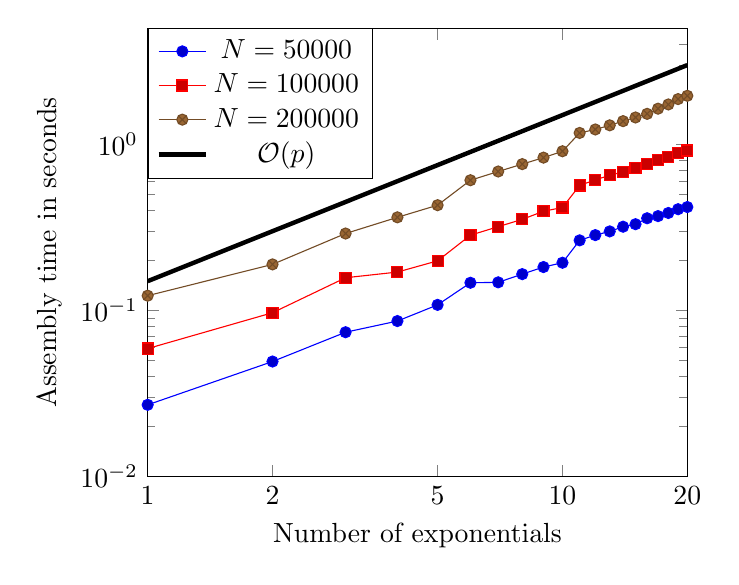
\begin{tikzpicture}
\begin{loglogaxis}[
	xlabel={Number of exponentials},
	ylabel={Assembly time in seconds},
	xmin=1, xmax=20,
	ymin=1e-2, ymax=5,
%	log x ticks with fixed point,
	xticklabel style={/pgf/number format/.cd,fixed,precision=2},
    xticklabel={%
      \pgfmathfloatparsenumber{\tick}%
      \pgfmathfloatexp{\pgfmathresult}%
      \pgfmathprintnumber{\pgfmathresult}%
	  },
	  xtick={1, 2, 5,  10, 20},
	  legend style={
	  	at={(0.0,1.0)},
		anchor=north west},
%	xticklabel=\pgfmathparse{10^\tick}\pgfmathprintnumber{\pgfmathresult}
]
%Fast N=50000
\addplot
coordinates{
(1, 0.027028) (2, 0.049254) (3, 0.07395) (4, 0.08631) (5, 0.108041) (6, 0.146784) (7, 0.147663) (8, 0.165446) (9, 0.182529) (10, 0.193782) (11, 0.264226) (12, 0.284138) (13, 0.299197) (14, 0.319235) (15, 0.330549) (16, 0.358907) (17, 0.36986) (18, 0.386211) (19, 0.406867) (20, 0.419369) 
};
\addlegendentry{$N=50000$}
%Fast N=100000
\addplot
coordinates{
(1, 0.05895) (2, 0.096882) (3, 0.157351) (4, 0.170255) (5, 0.198926) (6, 0.283903) (7, 0.319362) (8, 0.353572) (9, 0.395429) (10, 0.416635) (11, 0.565557) (12, 0.611283) (13, 0.650902) (14, 0.683053) (15, 0.718104) (16, 0.76064) (17, 0.804344) (18, 0.83463) (19, 0.883677) (20, 0.918114) 
};
\addlegendentry{$N=100000$}
%Fast N=200000
\addplot
coordinates{
(1, 0.122691) (2, 0.189373) (3, 0.290467) (4, 0.363561) (5, 0.430234) (6, 0.60801) (7, 0.686167) (8, 0.760237) (9, 0.831744) (10, 0.908682) (11, 1.1713) (12, 1.22885) (13, 1.3014) (14, 1.37929) (15, 1.45131) (16, 1.52625) (17, 1.63919) (18, 1.73834) (19, 1.87231) (20, 1.95994) 
};
\addlegendentry{$N=200000$}
%O(N) scaling
\addplot[ultra thick, no marks]
coordinates{
(1, 0.15) (20, 3)
};
\addlegendentry{$\mathcal{O}(p)$}
\end{loglogaxis}
\end{tikzpicture}
\end{document}